\documentclass[12pt,letterpaper] {report}
\usepackage{indentfirst}
\usepackage{titlesec}
\usepackage{titlecaps}
\usepackage{titletoc}
\usepackage[utf8]{inputenc}
\usepackage[margin=1in]{geometry}
\usepackage{blindtext}
\usepackage{graphicx}
\graphicspath{ {/Images/} }
\usepackage{setspace}
\usepackage{placeins}
\usepackage{hyperref}
\urlstyle{same}
\usepackage{multirow}
\usepackage{fancyhdr}
\usepackage{verbatim}
\usepackage{booktabs}
\usepackage{tabularx}
\usepackage{color,soul}
\usepackage{lastpage}

\renewcommand{\baselinestretch}{1.5} %double space document

\pagestyle{fancy} % Turn on the style
\fancyhf{} 
\rfoot{Page \thepage \hspace{1pt} of \pageref{LastPage}}
%\fancyfoot[R]{\thepage}

\fancypagestyle{plain}

\renewcommand{\headrulewidth}{0pt}
\titleformat
{\chapter} %command
[hang] %shape
{\normalfont\Large\bfseries} %format
{\thechapter.0} %label
{.5cm} %separation between chapter number and title
{\vspace{0.5cm}} %before-code vertical spacing
[\vspace{-1.5cm}] %after-code vertical spacing

\titleformat
{\section} %command
[hang] %shape
{\normalfont\bfseries\large} %format
{\thesection} %label
{0.5cm} %separation between chapter number and title
{\vspace{0cm}}


\begin{document}
\begin{titlepage}
	\centering % centers all content in scope
	{\scshape\huge Spiri Robotics \par}
	\vspace{1.5cm}
	
\includegraphics[width=0.15\textwidth]{SpiriLogo.png}\par\vspace{1cm}
	\vspace{1cm}
	{\huge\bfseries Product Design Document\par}
	\vspace{2cm}
	{\Large\itshape Adam Saule\par}
	\vfill
	% Bottom of the page
	{\large \today\par}
\end{titlepage}



\tableofcontents{}
\chapter{Background}
The purpose of this document is to record the design process for the Spiri Mu II Autonomous drone. This includes design requirements and constraints, design decisions, testing and prototyping, verification, and a user manual.
At the end of the document, drawings of the designs will be listed. Rendered images of the drone can be added later.
All the files associated with the document should be in their own folder.
\section{Introduction}

\section{Industry Background}


\chapter{Design Requirements}
There are several different quantities that need to be defined. These include:
\begin{itemize}
	\setlength{\itemsep}{0pt}%
	\setlength{\parskip}{-6pt}%
	\item Thrust to weight ratio
	\item Mass
	\item Dimensions
	\item Power requirements
	\item Flight duration
	\item Noise levels
	\item Water proofing 
\end{itemize}

 
\begin{table*}[ht]
	\centering
	\caption[Design Requirements]{\bfseries{Design Requirements}}
	\label{tab:require}
	\vspace{5pt}
	\begin{tabularx}{\textwidth}{Xll}	
		\toprule[2pt]
		\textbf{Requirement Identifier} & \textbf{Description} & \textbf{Priority}\\
		\toprule[2pt]
		A1 & Shall have a battery life of 1 hour & High\\
		\hline
		B1 & Shall have ... & Mid\\
		\hline
		C1 & Shall have ... & Low\\
		\hline
	\end{tabularx}
\end{table*}

The requirements for each component (from the following sections) should be listed here Table \ref{tab:require}. In the component selection section, an explanation for how each choice meets the requirement.

\chapter{Component Information}
This section details the definition, background information, and purpose for each component.
\section{Propulsion}
The motors and propellers work together to achieve a desired thrust. Many factors play into the amount of thrust, speed, and noise of the motor-propeller assembly. 

\subsection{Motor}
Brushless DC motors (BLDC) are the common motors used for quadcopter drones. 
Motor selection depends on required thrust, thrust depends on the total weight of the frame size. Generally, the thrust to weight ratio (TWR) in Equation \ref{eq1} is used to select a motor.
\begin{equation} \label{eq1}
TWR = \frac{T}{W}
\end{equation}
Where \textit{T} is the thrust and \textit{W} is weight, both in Newtons or pounds.

For the drone to be able to take off, a TWR $>$ 1 is required. Once the drone flies at an inclination, the thrust is split into x and y components. This means that the y-component of the thrust can drop. So for a TWR $ \geq $ 1.3 would be required for a maximum inclination angle of 40. In general, a TWR $ \geq $ 2.0 should be used at a minimum, so with 4 motors, each motor must provide a thrust equal to the mass divided by 4. (Cite quadcopter paper)

The constant velocity of a motor ($K_v$) is defined as the number of RPMs a motor will turn when 1V is applied with no load. 

\subsection{Propeller}
There are a couple of specifications that determine the performance of the propeller. Pitch, size, the number of blades; propeller material, and propeller weight \cite{droneomega}

The pitch of a propeller is defined as the distance the propeller would move in one revolution if it were moving through a soft solid. The higher the pitch, the faster the drone will fly. This is analogous to a screw; the pitch is measured the same way. The pitch must not be too flat or too steep as this will result in no lift being generated. 

\begin{figure}[!htb]
	\graphicspath{ {Images/} }
	\centering
	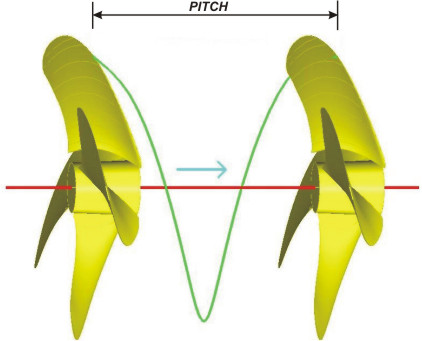
\includegraphics[width=0.6\textwidth,scale=0.8]{propeller.jpg}
	\caption{Propeller pitch }
	\label{fig:propeller}
\end{figure}

The length of the propeller from tip-to-tip is the defined as the length. Longer propellers generate more thrust for the same speed but require more torque from the motor. 

Number of blades - what effect does adding blades have?

Propeller material and weight - how does this affect performance? Noise? Would a smoother material be quieter? is noise caused by surface roughness or vibrations in the propeller along it's length?

\section{Chassis}
The chassis includes the internal frame, the arms, and the landing feet. 

Detail what characteristics each part of the chassis should have.

\hl{It might be helpful to develop a finite element model (FEM) of the top and bottom plates with the arms attached to determine optimal plate material and thickness.}

NOTE: Make a table comparing manufacturing techniques; 3D printing, injection moulding.

Look for other manufacturing techniques for landing gears and other common parts.

\subsection{Frame Design}
The size of the drone will depend on several factors. The size of the propellers, battery pack, and electronics. 
The frame of the drone will be constructed of 3D printed nylon parts because this allows for modularity and easy replacement of parts in the event of a failure. 
The top and bottom plates will compress the arms to hold them in place,  these plates will need to be stiff? (check) The arms need to be held in tight between the plates, we should consider adding some vibration damping between the plates to reduce transfer to the electrical components.

Why should their be a power and reset on the outside? Just quickly explain why.


\subsection{Arms}
Define what the arms are.

The arms must be long enough so that the frame does not hinder the function of the propulsion system. The arms must also be thin enough to ensure thrust is not reduced during operation. (not sure if this would make a big difference, could test in motor testing rig by placing different sized arms behind propeller and measure the drop in performance)

\subsection{Landing Feet}
Define what the landing feet are.

The feet could be placed in two different locations. Either beneath the motors at the end of the arms or near the body at the beginning of the arms. An analysis of the best location should be conducted with consideration placed on durability of body on hard landings and the landing platform. (Compare the two placements, pros and cons)

\section{Electronics}

\subsection{Computer and Carrier Board}
Define what the computer and carrier board do. 

What functions do they serve on the drone?

\subsection{Flight Controller}
Define what the flight controller does.

\subsection{Electronic Speed Controller}
The electronic speed controller (ESC) send pulse width modulation (PWM) signals to the motors to control the speed \hl{(source)}

\subsection{GNSS/Compass}
Define what the GNSS/Compass does.

\subsection{Optical Components}
Define what role the optical components do; image recognition, finding landmarks, determining the distance to objects, etc. 

The optical components are the cameras and the range finder.

\subsection{Power}

This includes the batteries and battery pack design. \\

Two types of lithium batteries are being considered, the lithium ion and lithium polymer batteries. Both have advantages and disadvantages compared to one another. \\

The major difference between lithium ion and lithium polymer batteries is the type of electrolyte used. LiPo batteries use a micro porous electrolyte as opposed to a liquid electrolyte and a porous separator. They also contain laminated sheets which eliminates the need for compression. Since the LiPo batteries don’t need compression, they can be made into other shapes, such as a “pouch”. They offer a slightly higher specific energy, but the manufacturing cost can be higher than traditional cylindrical batteries. Other than that, the two batteries are essentially the same. They both use the same cathode and anode material and have the same amount of electrolyte. \\

Lithium ion batteries vary depending on the type of material used as the cathode. \hl{(Elaborate on this, could influence which batteries will be used)} reference\\



\subsection{Power Management}
The power management system consists of the power distribution board... Is there more?



What does the power distribution board do?

\subsection{Modular Payloads}
A feature of the Spiri is that it can accommodate different payloads mounted on it's underside. (should include picture here) A \textbf{payload} is defined as an additional component added to the drone to serve a specific function.

\chapter{Component Selection}
This section details the process and reason for selecting each component
\section{Propulsion}

A testing rig should be designed to test the thrust of each motor-propeller assembly for two reasons:
\begin{enumerate}
	
	\item Ensures the motors are functioning
	\item Ensure the thrust from motor is within a certain tolerance
	
\end{enumerate}

An example rig can be found here, \href{https://www.banggood.com/Mayatech-MT10-10KG-Motor-Thrust-Tester-Propeller-Power-Tension-Measurement-For-RC-Model-Racing-Drone-p-1442104.html?gmcCountry=CA&currency=CAD&createTmp=1&utm_source=googleshopping&utm_medium=cpc_bgs&utm_content=yixuan&utm_campaign=ssc-ca-en-0213&gclid=CjwKCAjwmKLzBRBeEiwACCVihhjP9RAx65sLv2OFui5eUaMqfx3rBVgE6KZotZjVDXiZH75DfHi8yRoCh1EQAvD_BwE&cur_warehouse=CN}{motor testing rig}.

\subsection{Motor}
Include the desired motor specifications and possible products.
\subsection{Propeller}
There are a couple of specifications that determine the performance of the propeller. Pitch, size, the number of blades; propeller material, and propeller weight \cite{droneomega}

The pitch of a propeller is defined as the distance the propeller would move in one revolution if it were moving through a soft solid. The higher the pitch, the faster the drone will fly. This is analogous to a screw; the pitch is measured the same way. The pitch must not be too flat or too steep as this will result in no lift being generated. 

\begin{figure}[!htb]
	\graphicspath{ {Images/} }
	\centering
	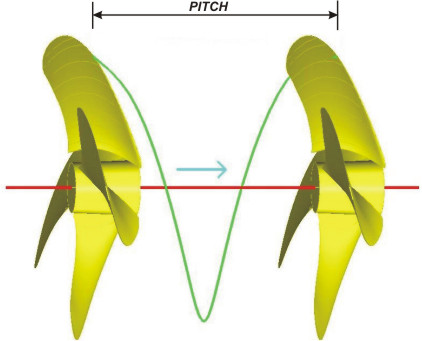
\includegraphics[width=0.6\textwidth,scale=0.8]{propeller.jpg}
	\caption{Propeller pitch }
	\label{fig:propeller}
\end{figure}

The length of the propeller from tip-to-tip is the defined as the length. Longer propellers generate more thrust for the same speed but require more torque from the motor. 

\section{Chassis}
The chassis includes the internal frame, the arms, and the landing feet. These will be made of various materials, most being 3D printed.

\hl{It might be helpful to develop a finite element model (FEM) of the top and bottom plates with the arms attached to determine optimal plate material and thickness.}

NOTE: Make a table comparing manufacturing techniques; 3D printing, injection moulding.

Look for other manufacturing techniques for landing gears and other common parts.

\subsection{Materials}
Table \ref{tab:material} shows the possible material properties which could be used for the chassis components. 

Other materials may be added and evaluated to determine if they are suitable for use in the drone. 

\begin{table*}[ht]
	\centering
	\caption[Material Properties]{\bfseries{Material properties for chassis}}
	\label{tab:material}
	\vspace{5pt}
	\begin{tabularx}{\textwidth}{Xp{2.5cm}p{2.5cm}p{2.5cm}}	
		\toprule[2pt]
		\textbf{Material} & \textbf{Density (g/cm$^3$)} & \textbf{Ultimate Strength (MPa)} & \textbf{Young’s Modulus (MPa)}\\
		\toprule[2pt]
		PA2200 Nylon – Laser Sintered & 0.93 & 48.0 & 1700 \\
		\hline
		PA1101 Nylon – Laser Sintered & 0.99 & 48.0 & 1600\\
		\hline
		PA12 Nylon – Multijet Fusion & 1.01 & 48.0 & 1800\\
		\hline
		Thermoplastic Polyurethane (TPU)$^1$ & 1.12 & 5.5 & 65 \\
		\hline
		Epoxy/Carbon Fiber Composite$^2$ & 1.4 & 878.0 & 94.6 \\
		\hline
	\end{tabularx}
\end{table*}
\noindent
$^1$This is an anisotropic material.\\
$^2$These are average values.

% need to add references

a military version could be made with a carbon fibre and kevlar blend, hardened with resin through vacuum. Propeller guards could be made the same way. 

\hl{Pros and cons of propeller guards?}

\subsection{Frame Design}
The size of the drone will depend on several factors. The size of the propellers, battery pack, and electronics. 
The frame of the drone will be constructed of 3D printed nylon parts because this allows for modularity and easy replacement of parts in the event of a failure. The type of nylon from Table \ref{tab:material} will be selected based on cost. 
The top and bottom plates will compress the arms to hold them in place,  these plates will need to be stiff? (check) and could be constructed from off the shelf carbon fiber sheets cut to the specified shape. The arms need to be held in tight between the plates, we should consider adding some vibration damping between the plates to reduce transfer to the electrical components. \hl{The manufacturer of these plates still needs to be determined.} 

Consideration should also be given to the placement of a power and reset button on the outside of the quadcopter.

\hl{List requirements for the frame design.}

\subsection{Arms}
The arms should be constructed from carbon fiber tubes. The sharp of the tubes will be selected based on the method selected to fix them to the frame, the strength of the tubes under bending, and the cost. The possible shapes are as follows:

\begin{itemize}
	\setlength{\itemsep}{0pt}%
	\setlength{\parskip}{-6pt}%
	\item Square – easier to fix to the frame and will not rotate, not as aesthetically pleasing
	\item Circular 
	\item Elliptical 
	\item Rectangular
\end{itemize}

The method for fixing the arms to the frame in order to prevent rotation is challenging. \hl{Ideas need to be generated and documented. }

\hl{List the requirements of the arms.}

\subsection{Landing Feet}
The intent in designing the landing feet is that they will be modular and can accommodate a variety of use cases. 

The feet could be placed in two different locations. Either beneath the motors at the end of the arms or near the body at the beginning of the arms. An analysis of the best location should be conducted with consideration placed on durability of body on hard landings and the landing platform.

\hl{List the different styles of feet.}

\hl{List the requirements of the feet.}

The landing feet should be 

\section{Electronics}

\subsection{Computer and Carrier Board}
The Spiri Mu uses a Nvidia TX2 for the computer and an \href{http://connecttech.com/product/asg002-elroy-carrier-for-nvidia-jetson-tx2-tx1/}{Elroy Carrier board}, which acts as a motherboard for the computer.

The reason for using this computer is it has a graphics processing unit on board so the image recognition algorithms can be run on the unit. 

ConnectTech will make the carrier board for the next generation Nvidia SOM. The new carrier board will incorporate camera input to remove the need for the camera interposers and ribbon cables. (source?)

\hl{Why was the connectech board selected?}

\subsection{Flight Controller}
The current flight controller used on the Spiri Mu is the \href{https://store.mrobotics.io/mRo-PixRacer-R14-Official-p/auav-pxrcr-r14-mr.htm}{mRo AUAV Pixracer R15}mRo AUAV Pixracer R15. The reason this was selected is …(I assume this is due to the compatibility with the GPS or vice versa)

This package contains:

\begin{itemize}
	\setlength{\itemsep}{0pt}%
	\setlength{\parskip}{-6pt}%
	\item Invensense ICM-20608-G 3-axis accelerometer/gyroscope
	\item Invensense MPU-9250 3-axis accelerometer/gyroscope/magnetometer 
	\item MEAS MS5611 barometer
	\item Honeywell HMC5983 magnetometer temperature compensated
\end{itemize}

\subsection{Electronic Speed Controller}
For small drones,  4-in-1 ESC's are appropriate. For larger drones \hl{(what does larger mean in this case?)}, one ESC per motor would be required \hl{(why? I assume more power output)} 

Large drones (in our case) may have 8 motors, one up and one down on each of four arms.

\subsection{GNSS/Compass}
The GPS and compass used on the Spiri Mu is the \href{https://store.mrobotics.io/mRo-GPS-u-Blox-Neo-M8N-Dual-Compass-LIS3MDL-IST831-p/mro-gps003-mr.htm}{mRo GPS u-Blox Neo-M8N}. 

For the next generation, the RTK GPS available from MRo, which greatly improves position accuracy. \hl{What are the differences from the current one? How much more accurate is it?}

\subsection{Optical Components}
The optical components are the cameras and the range finder.

The camera units currently used on the Spiri Mu is two \href{https://leopardimaging.com/product/cmos-sensor-modules/mipi-camera-modules/li-m021c-mipi/}{LI-M021C-MIPI} . Another camera unit is being considered which is the the AR0144 \hl{provide link}

An IR sensor could also be added to the array. \hl{what benefit does this provide}

The reason for this is that we want direct CSI input for the built in cameras, not a USB interface. \hl{what are the benefits to using CSI over USB?}

\subsection{Power}
The battery pack should incorporate a step-down converter and 5 cells. \hl{why 5 cells? why not 6 cells?}
\noindent
The battery pack should have the following characteristics:
\begin{itemize}
	\setlength{\itemsep}{0pt}%
	\setlength{\parskip}{-6pt}%
	\item Easily changed with a clip mechanism
	\item Connected to the drone using blade type connectors
	\item Fixed 15.5V
	\item Ability to supply 40A
	\item Spot welded connections between cells
	\item Balance charging
\end{itemize}

Hot-swapping batteries and moving batteries from one drone to the other should be possible.

\subsection{Power Management}
The power management system consists of the power distribution board.

\subsection{Modular Payloads}
\noindent
The drone will be designed to carry a variety of different payload masses. These could include:
\begin{itemize}
	\setlength{\itemsep}{0pt}%
	\setlength{\parskip}{-6pt}%
	\item FLIR Camera + gimbal
	\item Water testing equipment
	\item Normal camera + gimbal
	\item Agricultural multi-spectral sensor
	\item LIDAR
\end{itemize}
\hl{Need to know whether each needs a custom bottom shell}

\section{Overall Construction}
Overview of properties for the entire drone. \\

\hl{Would be a good idea to make requirements for each subsection then requirements for the overall drone.}\\

\hl{This section will include a wiring diagram to be added later.}\\
\chapter{Research of Similar Products}
These section is for research on similar products and how they designed their drone.
\chapter{Preliminary Design}
Explain first design and why the decisions were made for the selected parts.
\chapter{Prototyping \& Testing}

\chapter{Detailed Design}

\section{Design Overview}

\section{Electrical Design}

\subsection{Wiring Diagram}
\chapter{Verification \& Testing}

\chapter{Conclusion}

\begin{spacing}{2}
\renewcommand\bibname{References}
\begin{thebibliography}{1}
	\vspace{1cm}
	
	\bibitem{droneomega}
	DroneOmega. "Quadrocopter Propellers". 2020.[Online],	
	\textit{Available: https://www.droneomega.com/quadcopter-propeller/}
	
	\bibitem{propellerpages}
	Propeller Pages. "Propeller Pitch". 2020.[Online],	
	\textit{Available: http://www.propellerpages.com/?c=articles\&f=2006-03-08\_what\_is\_propeller\_pitch}
	
	\bibitem{pa2200}
	P. Formiga. "Material data sheet PA 2200". 2020. vol. 49, no. 0, pp. 1–2
	
	\bibitem{pa1101}
	“PA 1101 Product Texts EOS GmbH - Electro Optical Systems,” 2018.
	
	\bibitem{pa12}
	U.S. FDA, “HP 3D High Reusability PA 12,” pp. 3–4.
	
	\bibitem{tpu}
	“TPU Material Data Sheet,” vol. 49, no. 0, p. 9492, 2016.
	
	\bibitem{carbon}
	MatWeb, “Overview of materials for Epoxy / Carbon Fiber Composite MatWeb,” pp. 1–2.
	
	\bibitem{lipobat}
	“BU-205: Types of Lithium-ion.” [Online]. Available: .	
	\textit{Available: https://batteryuniversity.com/learn/article/types\_of\_lithium\_ion}


\end{thebibliography}
\end{spacing}

\end{document}
